\documentclass[12pt,a4paper]{article}
\usepackage{amsmath,amscd,amsbsy,amssymb,latexsym,url,bm,amsthm}
\usepackage{threeparttable}
\usepackage{epsfig,graphicx,subfigure}
\usepackage{enumitem,balance}
\usepackage{wrapfig}
\usepackage{float}
\usepackage{amsmath}
\usepackage{mathrsfs,euscript}
\usepackage[usenames]{xcolor}
\usepackage{hyperref}
\usepackage[vlined,ruled,linesnumbered]{algorithm2e}
\usepackage{array}
\hypersetup{colorlinks=true,linkcolor=black}

\newtheorem{theorem}{Theorem}
\newtheorem{lemma}[theorem]{Lemma}
\newtheorem{proposition}[theorem]{Proposition}
\newtheorem{corollary}[theorem]{Corollary}
\newtheorem{exercise}{Exercise}
\newtheorem*{solution}{Solution}
\newtheorem{definition}{Definition}
\theoremstyle{definition}

\renewcommand{\thefootnote}{\fnsymbol{footnote}}

\newcommand{\postscript}[2]
 {\setlength{\epsfxsize}{#2\hsize}
  \centerline{\epsfbox{#1}}}

\renewcommand{\baselinestretch}{1.0}

\setlength{\oddsidemargin}{-0.365in}
\setlength{\evensidemargin}{-0.365in}
\setlength{\topmargin}{-0.3in}
\setlength{\headheight}{0in}
\setlength{\headsep}{0in}
\setlength{\textheight}{10.1in}
\setlength{\textwidth}{7in}
\makeatletter \renewenvironment{proof}[1][Proof] {\par\pushQED{\qed}\normalfont\topsep6\p@\@plus6\p@\relax\trivlist\item[\hskip\labelsep\bfseries#1\@addpunct{.}]\ignorespaces}{\popQED\endtrivlist\@endpefalse} \makeatother
\makeatletter
\renewenvironment{solution}[1][Solution] {\par\pushQED{\qed}\normalfont\topsep6\p@\@plus6\p@\relax\trivlist\item[\hskip\labelsep\bfseries#1\@addpunct{.}]\ignorespaces}{\popQED\endtrivlist\@endpefalse} \makeatother

\begin{document}
\noindent

%========================================================================
\noindent\framebox[\linewidth]{\shortstack[c]{
\Large{\textbf{Lab09-Network Flow}}\vspace{1mm}\\
CS214-Algorithm and Complexity, Xiaofeng Gao \& Lei Wang, Spring 2021.}}
\begin{center}
\footnotesize{\color{red}$*$ If there is any problem, please contact TA Yihao Xie. }

\footnotesize{\color{blue}$*$ Name:Yanjie Ze  \quad Student ID:519021910706 \quad Email: zeyanjie@sjtu.edu.cn}
\end{center}

\begin{enumerate}
    \item  Consider there is a network consists $n$ computers. For some pairs of computers, a wire $i$ exists in the pair, which means these two computers can communicate with each other. When a signal passes through the wires, the noise in the signal will be amplified.If you know the magnification rate of noise $m_{i,j}$ of each wire (which must be greater than 1). Design an algorithm to find the route  for each other computer to send signals to the computer $v$ with the minimum total magnification rate of noise and analyze the time complexity.
    \begin{solution}
    ~\\
    The problem is essentially a single-source shortest paths problem, in which the computer $v$ is the source. 
    
    \textbf{The difference} lies in that in this problem, the edge amplifies the noise other than adding.
    
    Therefore, we propose an algorithm modified from $Dijkstra's\ Algorithm$ to solve this problem, just called $Dijkstra\ Modified$. The total algorithm is shown in Alg.~\ref{alg1}.
    
    \textbf{Denote:}
    \begin{itemize}
    \item
    Denote $V$ as the set of computers.
    \item
    Denote $E$ as the wires between computers.
        \item 
    Denote $d[u]$ as the magnification from the source computer $v$ to the computer $u$.
    \item
    Denote $Q$ as the min heap to extract the minimal value.
    \item
    Denote $S$ as the set to store the computers whose magnification from $v$ are known.
    \item Denote $w(u,m)$ as the magnification from $u$ to $m$.
        \end{itemize}

    \begin{algorithm}[H]
    \caption{Dijkstra Modified}\label{alg1}
    \For{$u\in V$}{
    \If{$u$ is $v$}
    {
        $d[u]=0$\;
    }
    \Else{$d[u]=\infty$\;}
    INSERT($Q,u$)\;
    }
    \While{$Q\neq \emptyset$}
    {
    $u\leftarrow$EXTRACT-MIN($Q$)\;
    $S\leftarrow S\cup \{u\}$\;
    \For{$m\in Adj[u]$}
    {
    \If {$d[m]>d[u]\times w(u,m) $}
    {
    $d[m]\leftarrow d[u]\times w(u,m)$\;
    DECREASE-KEY($Q,m$)\;
    }
    }
    }
    \end{algorithm}
    
 	For Alg.~\ref{alg1}:
	\begin{enumerate}
	    \item In line 1 to line 6, we initialize $d[u]$ and the heap $Q$.
	    \item In line 7 to line 8, we constantly extract the element from $Q$.
	    \item In line 10 to line 13, we do relaxation and use DECREASE-KEY operation to insert a new element.
	\end{enumerate}
	
	\textbf{Time Complexity}:
	
	The time complexity varies with different heap implementation, as show in table.~\ref{tab1}.
	
	\begin{table}[htbp]
	    \centering
	    \begin{tabular}{|c|c|c|c|}
	    \hline
	        Implementation &  EXTRACT-MIN & INS/DEC & $|V|\times$EXTRACT-MIN$+(|V|+|E|)\times$INS/DEC\\
	        \hline
	       Binary Heap  & $O(log|V|)$ & $O(log|V|)$ & $O((|V|+|E|)log|V|)$\\
	       Fibonacci Heap & $O(log|V|)*$ & $O(1)*$ & $O(|V|log|V|+|E|)$\\
	       \hline
	    \end{tabular}
	    \begin{tablenotes}
	    \footnotesize
	    \item
	    * means amortized analysis.
	    \end{tablenotes}
	    \caption{Time Complexity for Alg.~\ref{alg1}}
	    \label{tab1}
	\end{table}
	
    \end{solution}
	
	\item Suppose that we wish to maintain the transitive closure of a directed graph $G=(V,E)$ as we insert edges into $E$. That is, after each edge has been inserted, we want to update the transitive closure of the edges inserted so far. Assume that the graph $G$ has no edges initially and that we represent the transitive closure as a boolean matrix.
	\begin{enumerate}
	    \item Show how to update the transitive closure of a graph $G=(V,E)$ in $O(V^2)$ time when a new edge is added to $G$.
	    \begin{solution}
	    ~\\
	    Denote:
	    \begin{itemize}
	        \item 

	    Denote $N=\{1,2,...,|V|\}$ as the set of the numbers of vertexes.
	    \item
	    Denote the tuple $(i,j)$ as the edge from vertex $i$ to vertex $j$.
	    \item
	    Denote $t[i,j],1\leq i,j\leq |V|$ as the transitive closure matrix. $t[i,j]=1$ means vertex $i$ is connected to vertex $j$.
	    
	    
	    \textbf{Note:} If vertex $i$ is connected to vertex $j$, there exists a path along which a visitor from vertex $i$ can arrive at vertex $j$.
	    	    \end{itemize}
	    \textbf{Basic idea:} Whenever we add a new edge$(p,q)$, we need to check the vertexes that are connected to vertex $p$ and the vertexes that vertex $q$ is connected to, in order to update the matrix. Based on this, we propose Alg.~\ref{alg2}, \textbf{TC-Update}. 
	    
	    
	    
	   \begin{algorithm}[H]
	   \caption{TC-Update(p,q)}
	   \label{alg2}
	   \If{$t[p,q]==1$}{\Return \;}
	  \For{each $i$ in $N$}{
	  \For{each $j$ in $N$}{
	  \If{$t[i,p]==1$ and $t[q,j]==1$}{
	  $t[i,j]=1$\;
	  }
	  }
	  }
	   \end{algorithm}
	  
	   For Alg.~\ref{alg2}:
	   \begin{enumerate}
	       \item In line 1 to line 2, we update the value $t[p,q]$ in the matrix. If $t[p,q]$ has been updated, the algorithm returns back.
	       
	       \item In line 3 to line 6, We use a double-loop to update $t[i,j]$, if there exists a path.
	       
	   \end{enumerate}
	   
	   \textbf{Time Complexity}:$O(|V|^2)$
	   
	   Since there exists a double loop in Alg.~\ref{alg2}, the time complexity is $O(|V|^2)$.
	   
	   
	   
	   
	    \end{solution}
	    \item Give an example of a graph $G$ and an edge $e$ such that $\Omega(V^2)$ time is required to update the transitive closure after the insertion of $e$ into $G$, no matter what algorithm is used.
	    
	    \begin{solution}
~\\
        Consider that we want to insert an edge $(|V|,1)$ into the graph whose shape is a straight line:
        $$
        v_1 \rightarrow v_2 \rightarrow v_3 \rightarrow ... \rightarrow v_{|V|-1}\rightarrow v_{|V|}
        $$
        
        The transitive closure matrix $t_{|V|\times |V|}$ before inserting is:
        $$
        \begin{bmatrix}
        0 & 1&1 &...&1&1&1\\
        0 & 0&1 &...&1&1&1\\
        0 & 0&0 &...&1&1&1\\
        & & & ......& & &\\
        0 & 0&0 &...&0&0&1\\
        0 & 0&0 &...&0&0&0\\

        \end{bmatrix}
        $$
        
        Which has $\frac{|V|^2+|V|}{2}$ zeros.
        
        After we insert an edge $(|V|,1)$, the transitive closure matrix will become:
        $$
        \begin{bmatrix}
        1 & 1&1 &...&1&1&1\\
        1 & 1&1 &...&1&1&1\\
        1 & 1&1 &...&1&1&1\\
        & & & ......& & &\\
        1 & 1&1 &...&1&1&1\\
        1 & 1&1 &...&1&1&1\\
        \end{bmatrix}
        $$
        Which has all ones, meaning we need to change the values for $|V|^2-\frac{|V|^2+|V|}{2}$ times.
        
        Therefore, the time complexity is $\Omega (|V|^2)$.
	    \end{solution}
	    \item Describe an efficient algorithm for updating the transitive closure as edges are inserted into the graph. For any sequence of $m$ insertions, your algorithm should run in total time $\sum_{i=1}^m t_i=O(V^3)$, where $t_i$ is the time to update the transitive closure upon inserting the $i$th edge. Prove that your algorithm attains this time bound.
	    \begin{solution}
	    ~\\
	    In Alg.~\ref{alg2}, we find that there are some loops we can avoid, which is shown in Fig.~\ref{clousre} in detail. Then by adding some constraints, we can avoid some extra loops, which is shown in the new algorithm Alg.~\ref{alg3}. We first show the algorithm and explain this based on Fig.~\ref{clousre}.
	    
	    
	    
	    \begin{algorithm}[H]
	   \caption{TC-Update*(p,q)}
	   \label{alg3}
	   \If{$t[p,q]==1$}{\Return \;}
	  \For{each $i$ in $N$}{
	  \If{$t[i,p]==1$ and $t[i,q]!=1$}{
	  \For{each $j$ in $N$}{
	  \If{$t[q,j]==1$}{
	  $t[i,j]=1$\;
	  }
	  }
	  }
	  }
	   \end{algorithm}
	   
	   \textbf{So, why do we add these constraints ?}
	   
	   The whole process is shown in Fig.~\ref{clousre}. First, we judge whether $t[i,p]==1$ and $t[i,q]!=1$. When this is true, we can enter the next loop to find whether $t[q,j]==1$, then update $t[i,j]$. 
	   
	   Otherwise, if the judgement that $t[i,p]==1$ and $t[i,q]!=1$ is not true:
	   \begin{enumerate}
	       \item If $t[i,p]!=1$ and $t[i,q]==1$, adding $(p,q)$ will not change $t[i,j]$, which is only decided by $t[q,j]$.
	       \item If $t[i,p]!=1$ and $t[i,q]!=1$, adding $(p,q)$ will not change $t[i,j]$, which is not decided by all $p,q,j$.
	       \item If $t[i,p]==1$ and $t[i,q]==1$, adding $(p,q)$ will not change $t[i,j]$, which is decided by $t[i,j]$.
	       
	   \end{enumerate}
	   Therefore, we successfully avoid some extra loops by adding these constraints.
	   
	     \begin{figure}[htbp]
	        \centering
	        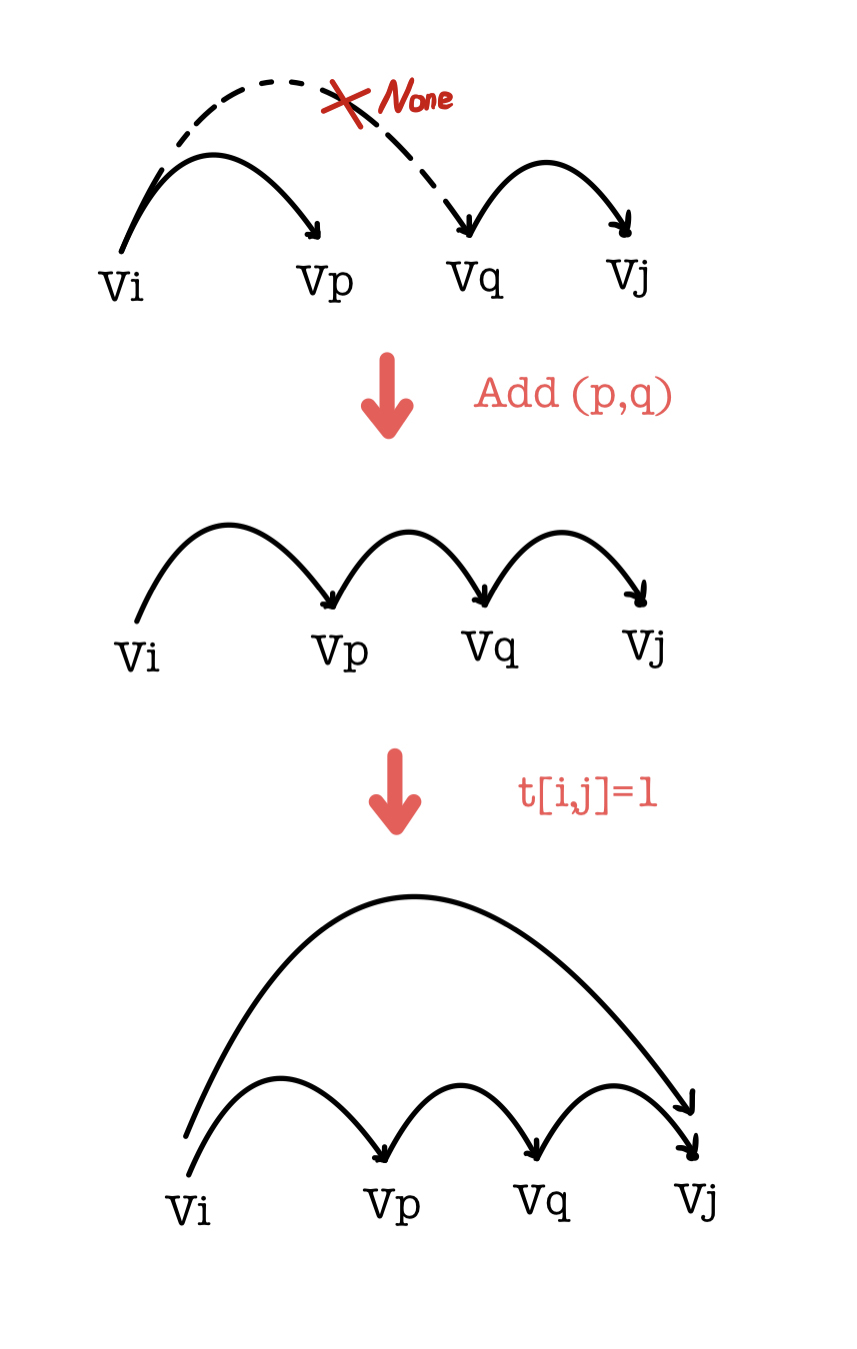
\includegraphics[width=6cm]{2.jpg}
	        \caption{Why Adding Constraints?}
	        \label{clousre}
	    \end{figure}
	    
	    
	   \textbf{Prove the time complexity is $O(|V|^3)$}:
	   
	   For $m$ insertions, since the number of edges is at most $|V|^2$, $m\leq |V|^2$.
	   
	   For the outer loop, the algorithm will be executed for $|V|$ times.
	   
	   While for the inner loop, which is in line 4 to line 7 in alg.~\ref{alg3}, the loop will be executed for at most $|V|^2$ times. This is because every time we enter this inner loop, we can change at least one value of the matrix. Thus, we at most enter this inner loop for $|V|^2$ times in total.
	   
	   Therefore, the total running time is $O(|V|^2\times |V| + |V|^2)=O(|V|^3)$.
	   
	   
	    \end{solution}
	\end{enumerate}

	
	
	\item An $n\times n$ grid is an undirected graph consisting of n rows and n columns of vertices, as shown in Figure 26.11. We denote the vertex in the $i$th row and the $j$th column by $(i,j)$. All vertices in a grid have exactly four neighbors, except for the boundary vertices, which are the points $(i,j)$ for which $i = 1, i = n, j = 1$, or $j = n$.
    Given $m\leqslant n^2$ starting points $(x_1,y_1), (x_2, y_2), ... , (x_m, y_m)$ in the grid, the escape problem is to determine whether or not there are $m$ vertex-disjoint paths from the starting points to any $m$ different points on the boundary such that every vertex in $V$ is included in at most one of the $m$ paths. For example, the grid in Figure \ref{Fig-EscapeProblem}(a) has an escape, but the grid in \ref{Fig-EscapeProblem}(b) does not.
    \begin{figure}[!htbp]
	\centering
	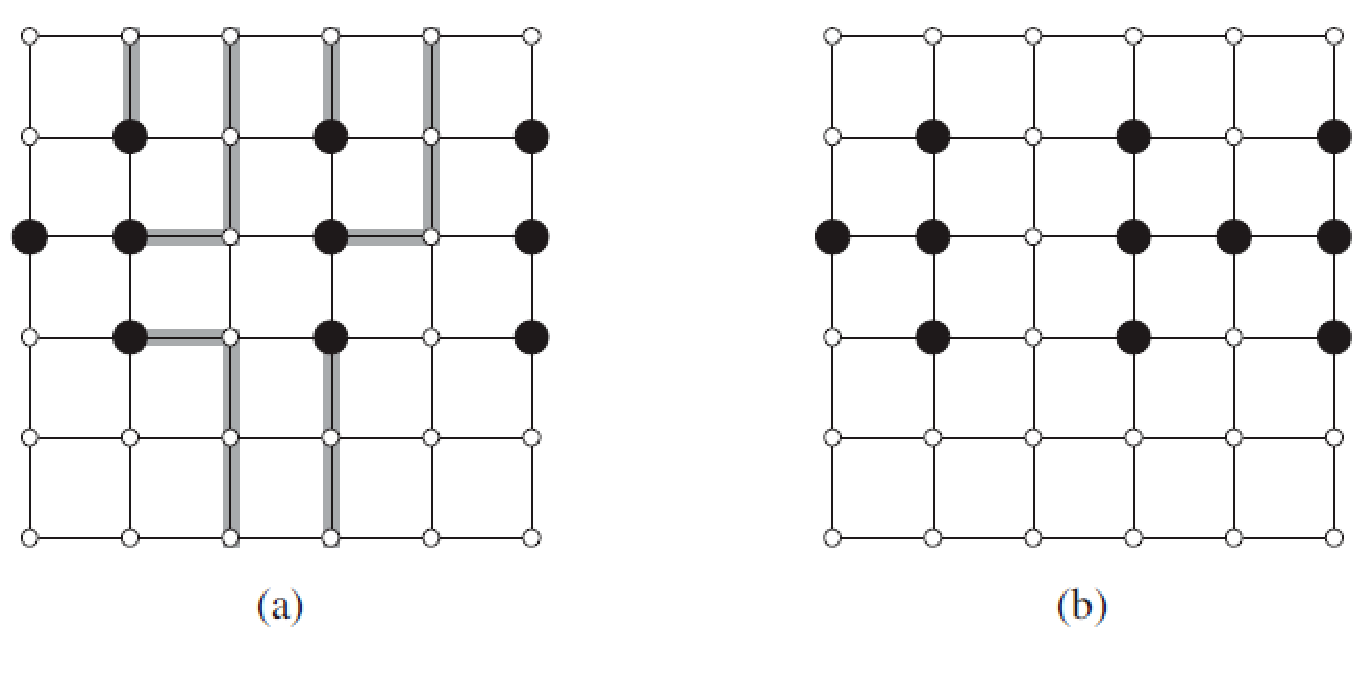
\includegraphics[width=0.5\textwidth]{Fig-EscapeProblem.pdf}
	\caption{Grids for the escape problem. Starting points are black, and other grid vertices are white. (a) A grid with an escape, shown by shaded paths. (b) A grid with no escape.}
	\label{Fig-EscapeProblem}
	\end{figure}
    \begin{enumerate}
        \item Consider a flow network in which vertices, as well as edges, have capacities. That is, the total positive flow entering any given vertex is subject to a capacity constraint. Show that determining the maximum flow in a network with edge and vertex capacities can be reduced to an ordinary maximum-flow problem on a flow network of comparable size. That is, the sizes of the two graph are in the same order of magnitude.
        \begin{solution}
        ~\\
        \textbf{Basic idea:}We can simply add an edge to represent the capacity of the vertex.
        
        We transform a vertex $v$ into two vertexes $v_{in}$ and $v_{out}$, and use an edge with the capacity equal to $v$ to connect them, as shown in Fig.~\ref{capcity vertex}. What's more, $v_{in}$ connects all entering edges and $v_{out}$ connects all departing edges.
        
        \begin{figure}[H]
            \centering
            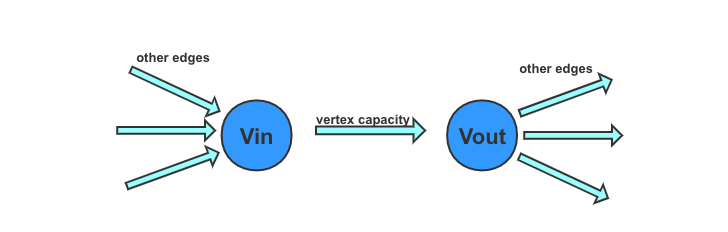
\includegraphics[width=15cm]{1.png}
            \caption{$v_{in},v_{out}$ with new edge}
            \label{capcity vertex}
        \end{figure}
        
        After this transformation, the problem turns into an ordinary maximum flow problem. We can solve this problem by \textbf{Ford-Fulkerson Algorithm}.
    ~\\
    
    Another problem is whether doing such transformation changes the order of magnitude of the graph.
    
    Assume the graph before transformation is $G_0=(V_0,E_0)$. 
    
    Denote the new graph is $G=(V,E)$.
    
    
    After transformation, each vertex except the source vertex is divided into 2 new vertexes, which means $|V|=2|V_0|$. And the number of edges becomes $|E|=|V_0|+|E_0|$.
    
    Therefore, the two graphs are in the same order of magnitude.
    
    
        
        
        \end{solution}
        \item Describe an efficient algorithm to solve the escape problem, and analyze its running time.
        \begin{solution}
        \textbf{Basic idea:} We can transform the escape problem into an ordinary maximum flow problem. Then it's easy to solve.
        
        ~\\
        First, we construct a graph by following these settings:
        \begin{enumerate}
        \item Create one source point $s_{start}$ and one end point $s_{end}$.
        
            \item For each starting point $s_i$, which is marked as \textbf{BLACK} in Fig.~\ref{Fig-EscapeProblem}: 
            \begin{enumerate}
                \item 
           $s_{start}$ is connected to $s_i$ with a directed edge $(s_{start}, s_i)$.
           \item
            $s_i$ is connected to the points $s_{other}$ it connects in Fig.~\ref{Fig-EscapeProblem} with  directed edges $(s_i, s_{other})$.
            
            
             \end{enumerate}
            \item For each boundary point $s_j$, which is on the \textbf{boundary} in Fig.~\ref{Fig-EscapeProblem}:
            \begin{enumerate}
                \item 
           $s_j$ is connected to $s_{end}$, with edge $(s_j, s_{start}$.
           \item
           Other points $s_{other}$ that are connected  to $s_j$ in Fig.~\ref{Fig-EscapeProblem} are connected to $s_j$ with directed edges $(s_{other}, s_j)$.
            \end{enumerate}
            
        \item For other points in Fig.~\ref{Fig-EscapeProblem}, they are inner points, and the connection between themselves is: For each two inner points $s_p,s_q$, connect them with two directed edges $(s_p,s_q)$ and $(s_q,s_p)$. 
        \item If one point is both a starting point and a boundary point, it is connected to both $s_{start}$ and $s_{end}$.
        \end{enumerate}
        After building such settings, we have initially constructed a graph, which is shown in Fig.~\ref{graph}.
        
        \begin{figure}[htbp]
            \centering
            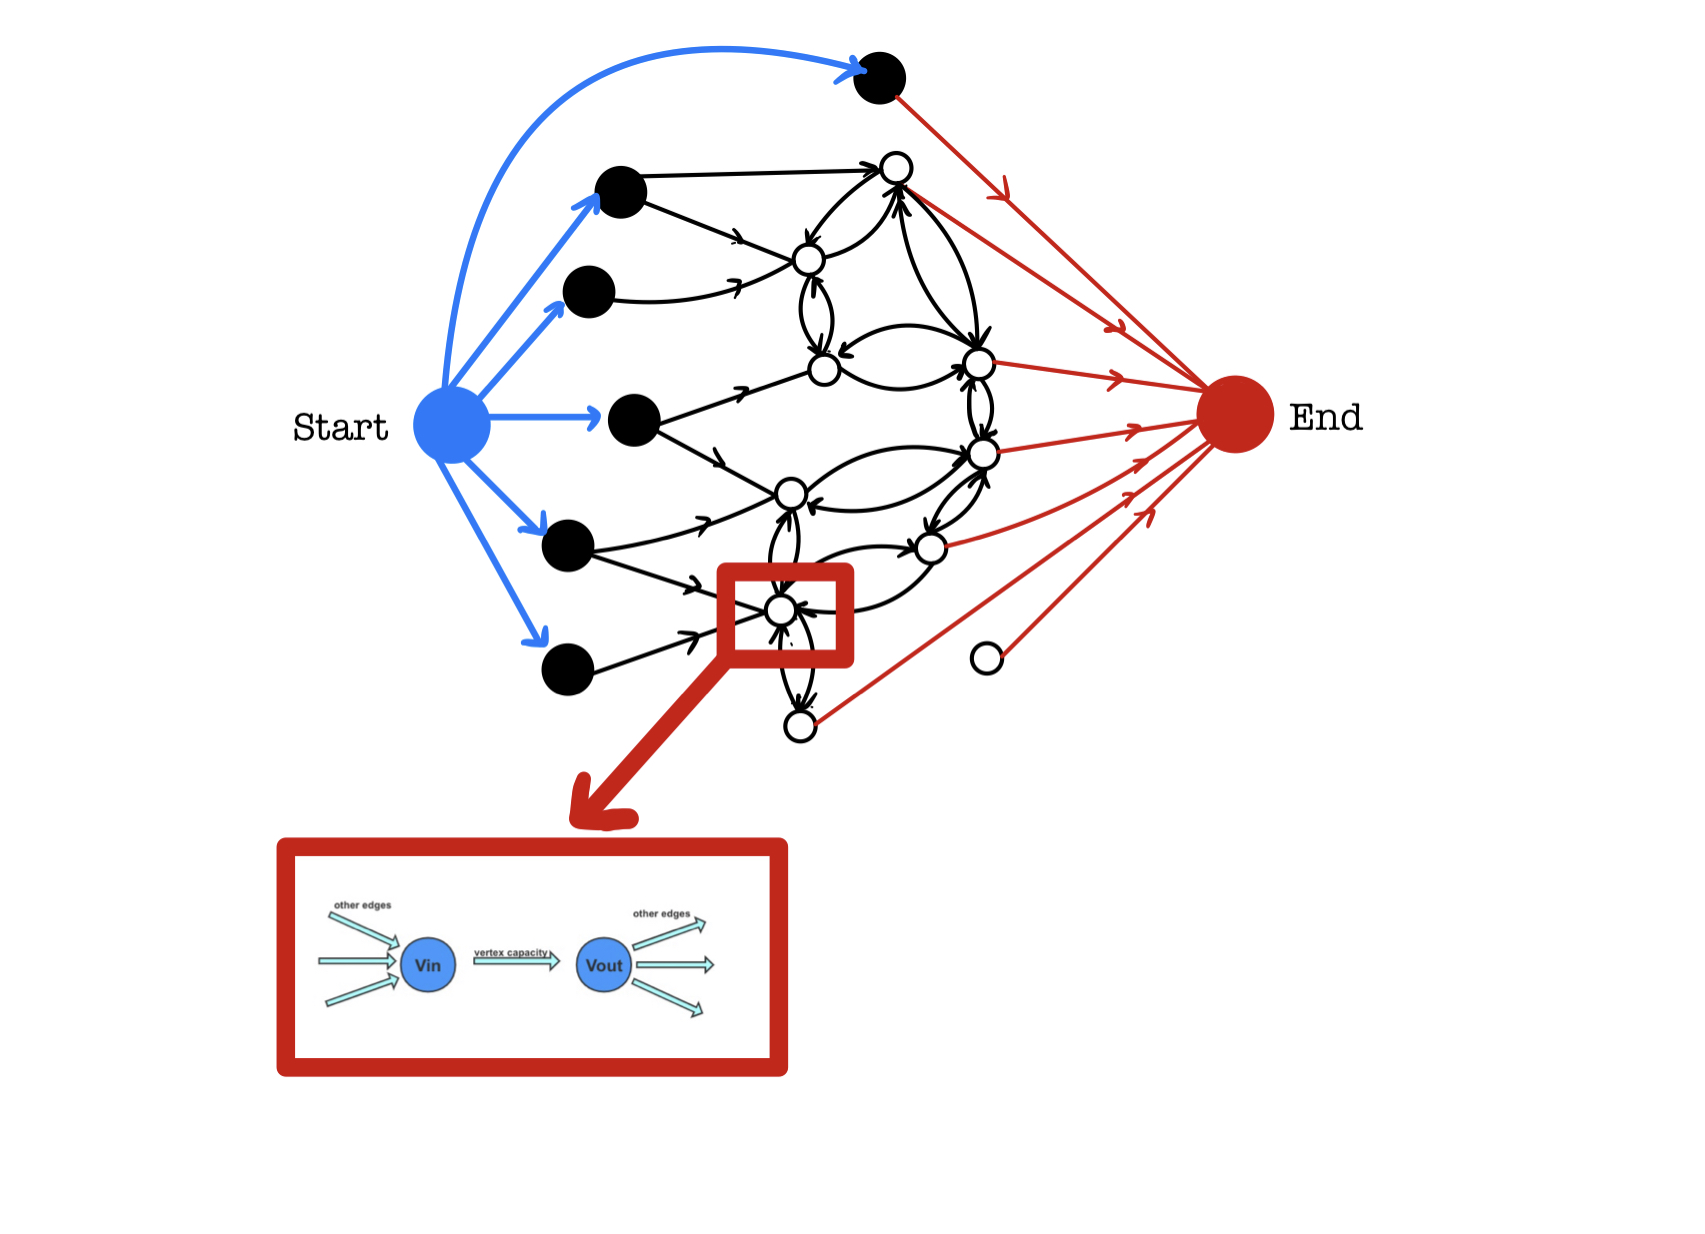
\includegraphics[width=13cm]{3.jpg}
            \caption{Graph Construction}
            \label{graph}
        \end{figure}
        
         Second, we transform this graph into a graph with the proper capacity.
    
    \begin{enumerate}
        \item Transform each inner point into two points$s_{in},s_{out}$, and add one edge between them, which has capacity \textbf{1}. This is the same as what we do in problem(a).
        \item Assign  other edges with capacity \textbf{1}.
    \end{enumerate}
    
    Finally, the problem is transformed into a maximum-flow problem, which can be solved by \textbf{Ford-Fulkerson Algorithm}.
    ~\\
    
    \textbf{Running Time for an $n\times n$ grid with $m$ starting points}:
    
    For the graph $G=(V,E)$ constructed by us:
    $$
    |V| = n^2 + 2
    $$
    $$
    |E| = (n-1)\times n + (n-1)\times n = 2n^2 - 2n
    $$
    And the maximum flow is:
    $$
    |f^*|\leq 4n-4
    $$
    Which is the number of all boundary points.
    
    Therefore, the running time is:
    $$
    T=O(|E|\times|f^*|)=O(n^3)
    $$
    
    
    
        \end{solution}
    \end{enumerate}
    
   
\end{enumerate}

\textbf{Remark:} Please include your .pdf, .tex files for uploading with standard file names.
\newpage


%========================================================================
\end{document}